\documentclass[conference]{IEEEtran}

% -----------------------------------------------------------------------
% Required Packages
% -----------------------------------------------------------------------
\usepackage{amsmath,amssymb,amsfonts}
\usepackage{graphicx}
\usepackage{textcomp}
\usepackage{xcolor}
\usepackage{booktabs}
\usepackage{cite}
\usepackage{microtype}
\usepackage{url}
\usepackage[hidelinks]{hyperref}

% -----------------------------------------------------------------------
% Float and Bibliography Spacing Adjustments (Strict <= 6-Page Budget)
% -----------------------------------------------------------------------
\setlength{\textfloatsep}{5pt plus 1pt minus 1pt}
\setlength{\floatsep}{5pt plus 1pt minus 1pt}
\setlength{\intextsep}{5pt plus 1pt minus 1pt}
\setlength{\dbltextfloatsep}{5pt plus 1pt minus 1pt}
\setlength{\dblfloatsep}{5pt plus 1pt minus 1pt}

% Compress bibliography inter-item spacing to eliminate orphan 7th page
\let\oldthebibliography\thebibliography
\let\endoldthebibliography\endthebibliography
\renewenvironment{thebibliography}[1]{%
  \begin{oldthebibliography}{#1}%
    \setlength{\itemsep}{1.2pt plus 0.4pt minus 0.2pt}%
    \setlength{\parskip}{0pt}%
}{%
  \end{oldthebibliography}%
}

% -----------------------------------------------------------------------
% Auto-Generated Empirical Macros (Generated from results/*.json)
% -----------------------------------------------------------------------
\newcommand{\AQThreshold}{7}
\newcommand{\AbideASDCount}{58}
\newcommand{\AbideSiteCount}{4}
\newcommand{\AbideTDCount}{62}
\newcommand{\AbideTotalAvailable}{157}
\newcommand{\AbideTotalSubjects}{120}
\newcommand{\AdolescentRawCount}{104}
\newcommand{\AdolescentRemovedCount}{7}
\newcommand{\AdolescentRetainedCount}{97}
\newcommand{\AdultLearningCurveMidAcc}{99.76}
\newcommand{\AdultLearningCurveMidN}{319}
\newcommand{\AdultLearningCurveMinAcc}{94.15}
\newcommand{\AdultLearningCurveMinN}{42}
\newcommand{\AdultRawCount}{704}
\newcommand{\AdultRemovedCount}{37}
\newcommand{\AdultRetainedCount}{667}
\newcommand{\AgeCorrPHolm}{0.1332}
\newcommand{\AgeCorrPRaw}{0.0444}
\newcommand{\AgeCorrR}{-0.1839}
\newcommand{\BalancedSiteChance}{25.00}
\newcommand{\BonferroniAlpha}{0.0056}
\newcommand{\ChildRawCount}{292}
\newcommand{\ChildRemovedCount}{30}
\newcommand{\ChildRetainedCount}{262}
\newcommand{\ConcordancePct}{100.0}
\newcommand{\ConformalCOneCovMean}{76.6}
\newcommand{\ConformalCOneCovSD}{9.0}
\newcommand{\ConformalCZeroCovMean}{94.4}
\newcommand{\ConformalCZeroCovSD}{3.3}
\newcommand{\ConformalEmptyRateMean}{10.2}
\newcommand{\ConformalEmptyRateSD}{3.6}
\newcommand{\ConformalEmptySumSevenPct}{59.8}
\newcommand{\ConformalEmptySumSixPct}{40.2}
\newcommand{\ConformalEmptySumsBorderlinePct}{100.0}
\newcommand{\ConformalMarginalCovMean}{89.8}
\newcommand{\ConformalMarginalCovSD}{3.6}
\newcommand{\ConformalRepCalN}{160}
\newcommand{\ConformalRepCoveredCOne}{32}
\newcommand{\ConformalRepCoveredCOnePct}{91.43}
\newcommand{\ConformalRepCoveredCZero}{96}
\newcommand{\ConformalRepCoveredCZeroPct}{96.97}
\newcommand{\ConformalRepCoveredTotal}{128}
\newcommand{\ConformalRepCoveredTotalPct}{95.52}
\newcommand{\ConformalRepEmptyCount}{6}
\newcommand{\ConformalRepQHat}{0.2574}
\newcommand{\ConformalRepTestN}{134}
\newcommand{\ConformalRepTotalCOne}{35}
\newcommand{\ConformalRepTotalCZero}{99}
\newcommand{\CovariateCombatAcc}{55.83}
\newcommand{\CovariateCombatCorrect}{67}
\newcommand{\CovariateRegressedAcc}{58.33}
\newcommand{\CovariateRegressedCorrect}{70}
\newcommand{\DiscordantCount}{0}
\newcommand{\LosoBalancedAcc}{54.67}
\newcommand{\LosoBinomialPOne}{0.158}
\newcommand{\LosoBinomialPTwo}{0.315}
\newcommand{\LosoBootstrapHigh}{64.17}
\newcommand{\LosoBootstrapLow}{46.67}
\newcommand{\LosoGlobalPermMean}{48.86}
\newcommand{\LosoGlobalPermP}{0.143}
\newcommand{\LosoGlobalPermSD}{5.45}
\newcommand{\LosoHeadlineAcc}{55.0}
\newcommand{\LosoHeadlineCorrect}{66}
\newcommand{\LosoHomogeneityChi}{7.640}
\newcommand{\LosoHomogeneityP}{0.0541}
\newcommand{\LosoPowerMDE}{62.7}
\newcommand{\LosoROCAUC}{0.6098}
\newcommand{\LosoTostP}{0.1355}
\newcommand{\LosoTostZOne}{3.303}
\newcommand{\LosoTostZTwo}{1.101}
\newcommand{\LosoWilsonHigh}{63.6}
\newcommand{\LosoWilsonLow}{46.1}
\newcommand{\LosoWithinPermMean}{50.18}
\newcommand{\LosoWithinPermP}{0.215}
\newcommand{\LosoWithinPermSD}{5.51}
\newcommand{\MajoritySiteBaseline}{41.67}
\newcommand{\MeanFDSD}{0.08}
\newcommand{\MeanFDVal}{0.14}
\newcommand{\MotionCorrPHolm}{0.2552}
\newcommand{\MotionCorrPRaw}{0.1276}
\newcommand{\MotionCorrR}{-0.1399}
\newcommand{\NumFmriVariants}{9}
\newcommand{\PreCombatSiteAcc}{73.33}
\newcommand{\PreCombatSiteBAcc}{67.17}
\newcommand{\PreCombatSiteSD}{5.00}
\newcommand{\QCHATThreshold}{4}
\newcommand{\RandomTenFoldAcc}{50.83}
\newcommand{\RandomTenFoldCorrect}{61}
\newcommand{\RawTotalCount}{2{,}154}
\newcommand{\RemovedDuplicatesCount}{278}
\newcommand{\RetainedTotalCount}{1{,}876}
\newcommand{\SexCorrPHolm}{0.8315}
\newcommand{\SexCorrPRaw}{0.8315}
\newcommand{\SexCorrR}{0.0196}
\newcommand{\SiteOnlyAcc}{52.50}
\newcommand{\SiteOnlyCorrect}{63}
\newcommand{\StudentAcc}{59.17}
\newcommand{\StudentCorrect}{71}
\newcommand{\StudentEdges}{50}
\newcommand{\StudentTeacherMcnemarP}{0.3018}
\newcommand{\StudentTeacherMcnemarStat}{1.0667}
\newcommand{\TeacherAcc}{55.00}
\newcommand{\TeacherEdges}{250}
\newcommand{\ToddlerRawCount}{1{,}054}
\newcommand{\ToddlerRemovedCount}{204}
\newcommand{\ToddlerRetainedCount}{850}
\newcommand{\TransductiveAcc}{56.67}
\newcommand{\TransductiveCorrect}{68}
\newcommand{\TransformerTestAcc}{45.83}
\newcommand{\TransformerTestCorrect}{55}
\newcommand{\TransformerTestP}{0.4114}
\newcommand{\TransformerTrainAcc}{82.50}
\newcommand{\UnharmonizedAcc}{57.50}
\newcommand{\UnharmonizedCorrect}{69}

% TODO tracking macro
\newcommand{\todo}[1]{\textcolor{red}{\textbf{[TODO: #1]}}}

\begin{document}

% -----------------------------------------------------------------------
% Title
% -----------------------------------------------------------------------
\title{A Methodological Audit and Reproducible Benchmark of Machine Learning for Autism Screening: Behavioral Tautologies, Scanner Generalization, and Uncertainty-Aware Decision Support}

% -----------------------------------------------------------------------
% Authors (Balanced Two-Column Author Block)
% -----------------------------------------------------------------------
\author{
\IEEEauthorblockN{Ratna Patil \\ Mohit Agrawal \\ Tanay Agrawal}
\IEEEauthorblockA{\textit{Dept. of Artificial Intelligence \& Data Science}\\
\textit{Vishwakarma Institute of Technology}\\
Pune, India\\
\{ratna.patil, mohit.agrawal24, tanay.agrawal24\}@vit.edu}
\and
\IEEEauthorblockN{Ayush Bagde \\ Shreyash Bhandare \\ Vibhav Bagade}
\IEEEauthorblockA{\textit{Dept. of Artificial Intelligence \& Data Science}\\
\textit{Vishwakarma Institute of Technology}\\
Pune, India\\
\{ayush.bagde24, shreyash.bhandare24, vibhav.bagade24\}@vit.edu}
}

\maketitle

% -----------------------------------------------------------------------
% Abstract (Strictly <= 200 words, no URL sentence)
% -----------------------------------------------------------------------
\begin{abstract}
Diagnostic latency in Autism Spectrum Disorder (ASD) often spans several years, motivating extensive research into machine learning screening using brief questionnaires and resting-state fMRI. However, published literature exhibits critical methodological vulnerabilities. This investigation presents a systematic methodological audit and reproducible benchmark across four public questionnaire cohorts (Adult, Adolescent, Child, Toddler; $N = \RetainedTotalCount$ total records) and an ABIDE-I multi-site resting-state fMRI cohort ($N = \AbideTotalSubjects$ subjects across four scanning centers). First, we show that widely reported near-perfect questionnaire classification reflects an arithmetic artifact: target labels in public repositories are deterministic functions of item response sums ($\sum_{i=1}^{10} A_i \ge \tau$, 100.0\% concordance), rendering machine learning non-incremental over standard scoring keys. Second, under Leave-One-Site-Out (LOSO) cross-validation with zero-calibration reference rescaling, functional connectivity models achieve \LosoHeadlineAcc\,\% accuracy (95\,\% CI: [\LosoWilsonLow\,\%, \LosoWilsonHigh\,\%]). Exact binomial tests ($p = 0.315$, two-sided) and within-site label permutations ($p = 0.215$, one-sided) indicate performance indistinguishable from chance under statistical power constraints (underpowered below \LosoPowerMDE\,\%). Third, split conformal prediction over 100 random splits provides \ConformalMarginalCovMean\,\% $\pm$ \ConformalMarginalCovSD\,\% marginal coverage while isolating borderline presentations (\ConformalCZeroCovMean\,\% controls vs. \ConformalCOneCovMean\,\% ASD). Edge deployment is left as future work.
\end{abstract}

\begin{IEEEkeywords}
Autism Spectrum Disorder, Methodological Audit, Label Leakage, ABIDE-I, Leave-One-Site-Out Cross-Validation, ComBat Harmonization, Conformal Prediction, Model Calibration, Edge Computing.
\end{IEEEkeywords}

% -----------------------------------------------------------------------
% Section I: Introduction
% -----------------------------------------------------------------------
\section{Introduction}

Autism Spectrum Disorder (ASD) is a neurodevelopmental condition characterized by persistent atypicalities in social communication, sensory processing, and restricted, repetitive patterns of behavior. Recent epidemiological surveillance by the Centers for Disease Control and Prevention (CDC) Autism and Developmental Disabilities Monitoring (ADDM) Network estimates ASD prevalence at 1 in 36 (2.7\,\%) among children aged 8 years in the United States \cite{maenner2023}. While early behavioral intervention improves longitudinal adaptive functioning, diagnostic latency between initial parental concern and specialist clinical confirmation regularly spans several years. This diagnostic backlog is driven by acute shortages of licensed clinicians certified to administer comprehensive evaluations, such as the Autism Diagnostic Observation Schedule, Second Edition (ADOS-2) \cite{lord2012ados}.

To facilitate earlier identification, extensive machine learning research has evaluated automated screening algorithms. Two primary computational paradigms dominate the literature: (i) supervised classification applied to brief caregiver- or self-report screening questionnaires, such as the 10-item Autism Spectrum Quotient (AQ-10) \cite{allison2012} and Quantitative Checklist for Autism in Toddlers (Q-CHAT-10), and (ii) functional connectivity classifiers trained on resting-state functional magnetic resonance imaging (rs-fMRI) blood-oxygen-level-dependent (BOLD) timeseries from multi-center repositories such as the Autism Brain Imaging Data Exchange (ABIDE-I) \cite{di2014}. Tabular questionnaire studies regularly report held-out test accuracies between 98.0\,\% and 100.0\,\% \cite{thabtah2018ijmi, raj2020}, while neuroimaging studies report cross-sectional diagnostic accuracies exceeding 70.0\,\% using autoencoders, graph neural networks, and transformer architectures \cite{heinsfeld2018, parisot2018, kan2022bnt, eslami2019}.

However, clinical translation of these computational models remains limited. In this investigation, we conduct an end-to-end methodological audit of both computational screening paradigms, identifying three critical vulnerabilities:
\begin{enumerate}
    \item \textbf{Circular Label Construction:} In public behavioral questionnaire benchmarks, diagnostic target classes are generated directly from deterministic cutoffs on item response sums. Supervised classifiers approximate this pre-existing arithmetic threshold rather than discovering latent clinical phenotypic signals.
    \item \textbf{Scanner Generalization and Evaluation Protocols:} In multi-site rs-fMRI benchmarks, cross-validation protocols heavily influence reported performance. Abraham et al. \cite{abraham2017} evaluated 871 subjects across 17 sites, reporting 67.0\,\% accuracy under leave-center-out cross-validation. In our class-balanced \AbideTotalSubjects-subject subset, random (non-site-held-out) CV yielded \RandomTenFoldAcc\,\% vs. LOSO \LosoHeadlineAcc\,\% (site-only baseline \SiteOnlyAcc\,\%), illustrating that small balanced subsets cannot test the broader generalization hypothesis.
    \item \textbf{Uncalibrated Point Estimates in Deployment:} Deployed screening tools frequently force binary classifications without rigorous uncertainty quantification, generating overconfident assertions on borderline presentations where clinical ambiguity is greatest.
\end{enumerate}

To address these vulnerabilities, we execute an empirical audit and formulate modular engineering prototypes for client-side decision support. We summarize our contributions as follows:
\begin{itemize}
    \item \textbf{Questionnaire Tautology Audit:} Across four developmental cohorts ($N = \RetainedTotalCount$ deduplicated records from an initial raw pool of $N = \RawTotalCount$), labels are an exact function of the item sum in all 1,876 retained records (\DiscordantCount\ discordant cases out of \RetainedTotalCount). Logistic regression matches the scoring rule (99.4--100\%); tree ensembles score 5--14 points below it.
    \item \textbf{Multi-Site Neuroimaging Benchmark:} On an ABIDE-I cohort across four scanning centers ($N = \AbideTotalSubjects$), we evaluate resting-state connectomes under strict Leave-One-Site-Out (LOSO) cross-validation with zero-calibration reference rescaling (\LosoHeadlineAcc\,\% accuracy, Wilson 95\,\% CI: [\LosoWilsonLow\,\%, \LosoWilsonHigh\,\%], bootstrap 95\,\% CI: [\LosoBootstrapLow\,\%, \LosoBootstrapHigh\,\%]). Statistical power analysis (minimum detectable accuracy \LosoPowerMDE\,\% at $80\,\%$ power), exact binomial tests ($p = \LosoBinomialPTwo$, two-sided), and 1,000 within-site label permutations ($p = \LosoWithinPermP$, one-sided) show performance indistinguishable from chance under power constraints, while a catalogue of \NumFmriVariants\ exploratory fMRI tests demonstrates that top-performing variants (\StudentAcc\,\%) are expected under multiple looks from the null ($\alpha_{\text{Bonf}} = \BonferroniAlpha$).
    \item \textbf{Modular Client-Side Decision Support Prototypes:} We explore modular client-side decision support: an inductive split conformal prediction layer evaluated over 100 random splits on tabular screening (\ConformalMarginalCovMean\,\% $\pm$ \ConformalMarginalCovSD\,\% marginal coverage; \ConformalCZeroCovMean\,\% controls vs. \ConformalCOneCovMean\,\% ASD) that flags borderline presentations ($\sum A_i \in \{6, 7\}$) as uncertain. Edge deployment is left as future work.
\end{itemize}
We will release evaluation scripts and preprocessing pipelines at \url{https://github.com/Mohit-ccreate/autism}.

% -----------------------------------------------------------------------
% Section II: Related Work
% -----------------------------------------------------------------------
\section{Related Work}

\subsection{Behavioral Questionnaire Screening}
The AQ-10 instrument was developed by Allison et al. \cite{allison2012} via psychometric item reduction from the full 50-item Autism Spectrum Quotient. In their clinical validation across 1,000 clinic cases and 3,000 controls, an integer referral cutoff of $\sum A_i \ge 6$ yielded 0.88 sensitivity and 0.91 specificity in adults, 0.93 sensitivity and 0.95 specificity in adolescents, and 0.95 sensitivity and 0.97 specificity in children. For toddlers, Allison et al. \cite{allison2012} evaluated the Q-CHAT-10, validating a clinical referral cutoff of $\sum A_i \ge 3$ (0.91 sensitivity, 0.89 specificity). 

Subsequent computational studies evaluated tabular classification algorithms on datasets released through the UCI Machine Learning Repository \cite{uci_adult, uci_adolescent, uci_child} and Kaggle \cite{thabtah2018toddler}, reporting near-perfect accuracy: Raj and Masood \cite{raj2020} reported 98.6\,\% accuracy on Adult AQ-10 using random 80/20 train/test splits, while Thabtah et al. \cite{thabtah2018ijmi} reported 99.7\,\% accuracy using 10-fold cross-validation. 

\subsection{Resting-State fMRI Connectomics on ABIDE-I}
The ABIDE-I consortium \cite{di2014} aggregated resting-state fMRI scans across 17 independent international imaging sites. Early deep learning investigations pooled subjects across sites under random 10-fold cross-validation, reporting 70.0\,\% accuracy with stacked autoencoders \cite{heinsfeld2018}, 70.3\,\% with ASD-DiagNet \cite{eslami2019}, and 73.2\,\% with the Brain Network Transformer \cite{kan2022bnt}. 

Abraham et al. \cite{abraham2017} evaluated multi-site resting-state fMRI on 871 subjects across 17 sites, reporting 67.0\,\% accuracy under leave-center-out cross-validation. Table~\ref{tab:literature_audit} summarizes these benchmarks with neutral facts from published papers.

\begin{table*}[t]
\centering
\caption{Literature Benchmark Overview Across Behavioral Questionnaire and Multi-Site Resting-State fMRI Modalities.}
\label{tab:literature_audit}
\footnotesize
\setlength{\tabcolsep}{5pt}
\resizebox{\textwidth}{!}{%
\begin{tabular}{lllll}
\toprule
\textbf{Study} & \textbf{Modality} & \textbf{Dataset \& $N$} & \textbf{Split Protocol} & \textbf{Reported Metric} \\
\midrule
Raj \& Masood (2020) \cite{raj2020} & Tabular (AQ-10) & Adult ($N = 704$) & Random 80/20 Train/Test & 98.6\,\% Acc. \\
Thabtah et al. (2018) \cite{thabtah2018ijmi} & Tabular (AQ-10) & Adult ($N = 704$) & 10-Fold Cross-Validation & 99.7\,\% Acc. \\
Heinsfeld et al. (2018) \cite{heinsfeld2018} & rs-fMRI (ABIDE-I) & 17 Sites ($N = 1{,}035$) & Random 10-Fold CV & 70.0\,\% Acc. \\
Eslami et al. (2019) \cite{eslami2019} & rs-fMRI (ABIDE-I) & 17 Sites ($N = 1{,}035$) & Random 10-Fold CV & 70.3\,\% Acc. \\
Kan et al. (2022) \cite{kan2022bnt} & rs-fMRI (ABIDE-I) & 17 Sites ($N = 1{,}009$) & 5-Fold Stratified CV & 73.2\,\% Acc. \\
Abraham et al. (2017) \cite{abraham2017} & rs-fMRI (ABIDE-I) & 17 Sites ($N = 871$) & Leave-Center-Out (17 Sites) & 67.0\,\% Acc. \\
\bottomrule
\end{tabular}%
}
\end{table*}

% -----------------------------------------------------------------------
% Section III: Methodology
% -----------------------------------------------------------------------
\section{Methodology}

\subsection{Behavioral Questionnaire Ingestion and Deduplication}
We audited four developmental cohorts from public repositories: UCI Adult ($N = \AdultRawCount$) \cite{uci_adult}, UCI Adolescent ($N = \AdolescentRawCount$) \cite{uci_adolescent}, UCI Child ($N = \ChildRawCount$) \cite{uci_child}, and Kaggle Toddler ($N = \ToddlerRawCount$) \cite{thabtah2018toddler}, comprising an initial pool of $N = \RawTotalCount$ records. Deduplication across the standardized key $[A_1, \dots, A_{10}, \text{Age}, \text{Sex}, \text{Target}]$ removed \AdultRemovedCount\ adult, \AdolescentRemovedCount\ adolescent, \ChildRemovedCount\ child, and \ToddlerRemovedCount\ toddler duplicates, yielding $N = \RetainedTotalCount$ unique retained participant records after removing $\RemovedDuplicatesCount$ duplicates (Table~\ref{tab:cohort_dedup}).

\begin{table}[t]
\centering
\caption{Behavioral Questionnaire Ingestion and Deduplication Breakdown.}
\label{tab:cohort_dedup}
\footnotesize
\setlength{\tabcolsep}{3.5pt}
\resizebox{\columnwidth}{!}{%
\begin{tabular}{lcccc}
\toprule
\textbf{Cohort} & \textbf{Raw $N$} & \textbf{Removed} & \textbf{Retained} & \textbf{Deduplication Key} \\
\midrule
Adult (AQ-10) \cite{uci_adult} & \AdultRawCount & \AdultRemovedCount & \AdultRetainedCount & $[A_1, \dots, A_{10}, \text{Age}, \text{Sex}, \text{Target}]$ \\
Adolescent (AQ-10) \cite{uci_adolescent} & \AdolescentRawCount & \AdolescentRemovedCount & \AdolescentRetainedCount & $[A_1, \dots, A_{10}, \text{Age}, \text{Sex}, \text{Target}]$ \\
Child (AQ-10) \cite{uci_child} & \ChildRawCount & \ChildRemovedCount & \ChildRetainedCount & $[A_1, \dots, A_{10}, \text{Age}, \text{Sex}, \text{Target}]$ \\
Toddler (Q-CHAT-10) \cite{thabtah2018toddler} & \ToddlerRawCount & \ToddlerRemovedCount & \ToddlerRetainedCount & $[A_1, \dots, A_{10}, \text{Age}, \text{Sex}, \text{Target}]$ \\
\midrule
\textbf{Total} & \textbf{\RawTotalCount} & \textbf{\RemovedDuplicatesCount} & \textbf{\RetainedTotalCount} & \textbf{Narrow-key matching} \\
\bottomrule
\end{tabular}%
}
\end{table}

\subsection{Tautology Verification and Scoring Rules}
We evaluated whether target columns represent arithmetic transformations of item responses. For each record, let $A_i \in \{0, 1\}$ denote the binary response for item $i \in \{1, \dots, 10\}$, and let $S = \sum_{i=1}^{10} A_i$ denote the integer sum. We defined the \textit{Benchmark Scoring Rule}:
\begin{equation}
\hat{y}_{\text{rule}} = \mathbb{I}(S \ge \tau)
\end{equation}
where $\tau$ is an integer threshold. In clinical validation by Allison et al. \cite{allison2012}, the validated clinical referral cutoff is $\tau = 6$ for AQ-10 and $\tau = 3$ for Q-CHAT-10. However, in the public repository target columns, labels follow $\tau \ge \AQThreshold$ for Adult, Adolescent, and Child, and $\tau \ge \QCHATThreshold$ for Toddler, inferred from concordance analysis (dataset documentation does not state the rule). 
We evaluated two feature variants across all classifiers: Variant A (items only: $\mathbf{x}_A = [A_1, \dots, A_{10}]^T \in \{0, 1\}^{10}$) and Variant B (items and demographics: $\mathbf{x}_B = [A_1, \dots, A_{10}, \text{Age}, \text{Sex}, \text{Jaundice}, \text{Family ASD}]^T$).
We also evaluated ensemble meta-learning via Stacking Generalization \cite{wolpert1992} combining linear and tree-based learners, and calibrated predicted probabilities using temperature scaling \cite{guo2017} minimizing Negative Log-Likelihood (NLL).

\subsection{ABIDE-I Cohort Selection and Connectome Extraction}
We obtained resting-state fMRI scans from the ABIDE-I preprocessed release \cite{craddock2013pcp} using the Configurable Pipeline for the Analysis of Connectomes (CPAC) with band-pass filtering ($0.01$--$0.1$~Hz) and global signal regression. We extracted BOLD timeseries across $V = 200$ regions of interest (ROIs) from the Craddock-200 (CC200) functional clustering atlas \cite{craddock2012}. For each subject, the functional connectivity matrix $\mathbf{R} \in \mathbb{R}^{200 \times 200}$ was computed via pairwise Pearson correlation:
\begin{equation}
R_{ij} = \frac{\sum_{t=1}^T (s_{i,t} - \bar{s}_i)(s_{j,t} - \bar{s}_j)}{\sqrt{\sum_{t=1}^T (s_{i,t} - \bar{s}_i)^2} \sqrt{\sum_{t=1}^T (s_{j,t} - \bar{s}_j)^2}}
\end{equation}
Upper-triangular off-diagonal elements were extracted and Fisher $z$-transformed, producing $D = V(V-1)/2 = 19,900$ edge features:
\begin{equation}
z_{ij} = \frac{1}{2} \ln \left( \frac{1 + R_{ij}}{1 - R_{ij}} \right)
\end{equation}

Table~\ref{tab:site_parameters} details the acquisition centers. Subjects were retrieved from four scanning centers (OHSU, OLIN, PITT, SDSU) by matching complete CC200 timeseries extracts and class balance within each site cache, retaining $N = \AbideTotalSubjects$ subjects from \AbideTotalAvailable\ available scans (\AbideASDCount\ ASD and \AbideTDCount\ TD). Across all \AbideTotalSubjects\ subjects, head motion was evaluated retrospectively post-hoc; mean framewise displacement was $\MeanFDVal \pm \MeanFDSD$~mm ($0.12 \pm 0.09$~mm for subjects with $FD \le 0.5$~mm \cite{power2014methods}). Prospective clinical screening pipelines require automated head-motion scrubbing and volume censoring criteria.

\begin{table}[t]
\centering
\caption{ABIDE-I Site Acquisition Parameters and Cohort Breakdown.}
\label{tab:site_parameters}
\footnotesize
\setlength{\tabcolsep}{2.5pt}
\resizebox{\columnwidth}{!}{%
\begin{tabular}{llccccc}
\toprule
\textbf{Site} & \textbf{Scanner Hardware} & \textbf{TR (ms)} & \textbf{ABIDE} & \textbf{Retained} & \textbf{ASD} & \textbf{TD} \\
\midrule
OHSU & Siemens Tim Trio 3T & 2500 & 28 & 25 & 12 & 13 \\
OLIN & Siemens Allegra 3T  & 1500 & 36 & 28 & 14 & 14 \\
PITT & Siemens Allegra 3T  & 1500 & 57 & 50 & 24 & 26 \\
SDSU & GE MR750 3T         & 2000 & 36 & 17 & 8  & 9  \\
\midrule
\textbf{Total} & \textbf{4 Scanning Centers} & \textbf{--} & \textbf{157} & \textbf{120} & \textbf{58} & \textbf{62} \\
\bottomrule
\end{tabular}%
}
\end{table}

\subsection{Cross-Site Generalization and ComBat Harmonization}
To evaluate out-of-scanner generalizability, we employed Leave-One-Site-Out (LOSO) cross-validation across the four scanning centers. In each LOSO fold, three acquisition centers formed the training set $\mathcal{D}_{\text{train}}$, while the remaining unseen center served as the test set $\mathcal{D}_{\text{test}}$.

We evaluated ComBat neuroimaging harmonization \cite{johnson2007combat} to adjust for additive and multiplicative site shifts. For feature $g$ in subject $j$ at training site $i$, the model assumes:
\begin{equation}
y_{ijg} = \alpha_g + \mathbf{X}_{ij}\boldsymbol{\beta}_g + \gamma_{ig} + \delta_{ig}\epsilon_{ijg}
\end{equation}
Harmonized training features are obtained via empirical Bayes estimates:
\begin{equation}
y_{ijg}^{\text{ComBat}} = \frac{y_{ijg} - \hat{\alpha}_g - \mathbf{X}_{ij}\hat{\boldsymbol{\beta}}_g - \hat{\gamma}_{ig}^*}{\hat{\delta}_{ig}^*} + \hat{\alpha}_g + \mathbf{X}_{ij}\hat{\boldsymbol{\beta}}_g
\end{equation}

For an unseen test site $k \notin \mathcal{S}_{\text{train}}$, site-specific batch shifts $(\gamma_{kg}, \delta_{kg})$ cannot be estimated without test site calibration data. To avoid test leakage, we implemented \textit{zero-calibration reference rescaling}:
\begin{equation}
y_{kjg}^{\text{unseen}} = \left( \frac{y_{kjg} - \hat{\alpha}_g}{\hat{\sigma}_{g,\text{pooled}}} \right) \hat{\sigma}_{g,\text{ref}} + \hat{\alpha}_g
\end{equation}
This rescales unseen test data to the reference training variance without updating site parameters. We also evaluated three alternative protocols: (a) unharmonized raw features (`none`), (b) transductive unlabeled standardization (standardizing the test center by its own unlabeled empirical mean and variance), and (c) covariate-aware ComBat adjusting for age, sex, and mean framewise displacement. In all pipelines, feature selection (ANOVA $F$-test, $K = \TeacherEdges$ edges) and classifier regularization were tuned strictly by nested cross-validation on $\mathcal{D}_{\text{train}}$ only.

\subsection{Knowledge Distillation to Compact Student Model}
To assess whether high-capacity representations can be compressed for low-latency decision support, we distilled functional connectivity features into a lightweight linear student model operating on $M = \StudentEdges$ top-ranked edges \cite{hinton2015}. For each LOSO fold, an in-fold teacher model produced softened probability predictions $p_T(\mathbf{x}) = \sigma(z_T / T)$ at temperature $T = 2.0$. The student model was trained inside the fold using a combined cross-entropy and mean-squared distillation objective:
\begin{equation}
\mathcal{L}_{\text{distill}} = (1 - \lambda)\mathcal{L}_{\text{CE}}(y, \sigma(z_S)) + \lambda T^2 \frac{1}{N} \sum_{i=1}^N (p_T(\mathbf{x}_i) - p_S(\mathbf{x}_i))^2
\end{equation}
with $\lambda = 0.5$. Hyperparameters were tuned exclusively on training sites.

% -----------------------------------------------------------------------
% Section IV: Empirical Results
% -----------------------------------------------------------------------
\section{Empirical Results}

\subsection{Questionnaire Tautology Audit}
Table~\ref{tab:questionnaire_audit} reports performance across repeated $5 \times 10$ stratified cross-validation on the deduplicated cohorts. The Benchmark Scoring Rule ($\sum A_i \ge \AQThreshold$ for AQ-10, $\sum A_i \ge \QCHATThreshold$ for Q-CHAT-10) achieves \ConcordancePct\,\% concordance across all four cohorts (\DiscordantCount\ discordant cases out of $\RetainedTotalCount$ records). 

Supervised classifiers (Logistic Regression, LightGBM \cite{ke2017lightgbm}, XGBoost \cite{chen2016xgboost}, CatBoost \cite{prokhorenkova2018catboost}) achieve 85.7\,\% to 100.0\,\% accuracy on Variant A. Logistic regression matches the scoring rule (99.4--100\%); tree ensembles score 5--14 points below it. We hypothesize this reflects axis-aligned splits approximating a diagonal boundary; we did not test this beyond a depth sweep. On Variant B, adding demographic covariates (age, sex, jaundice, family history) does not improve classification accuracy, because the ground truth label is fully determined by the item responses alone.

\begin{table*}[t]
\centering
\caption{Audit of Behavioral Questionnaire Screening: Benchmark Scoring Rule vs. Supervised Machine Learning Models (Repeated $5 \times 10$ Stratified CV).}
\label{tab:questionnaire_audit}
\footnotesize
\renewcommand{\arraystretch}{0.88}
\setlength{\tabcolsep}{3.5pt}
\resizebox{\textwidth}{!}{%
\begin{tabular}{llcccccc}
\toprule
\textbf{Cohort} & \textbf{Model / Protocol} & \textbf{Accuracy (\%)} & \textbf{Sensitivity} & \textbf{Specificity} & \textbf{ROC-AUC} & \textbf{Brier Score \cite{brier1950}} & \textbf{ECE} \\
\midrule
\textbf{Adult} & \textbf{Benchmark Scoring Rule ($\tau = 7$)} & \textbf{100.00 $\pm$ 0.00} & \textbf{1.000 $\pm$ 0.000} & \textbf{1.000 $\pm$ 0.000} & \textbf{1.000 $\pm$ 0.000} & \textbf{0.0000} & \textbf{0.0000} \\
($N = 667$) & Logistic Regression (Var A) & 99.96 $\pm$ 0.18 & 0.998 $\pm$ 0.007 & 1.000 $\pm$ 0.000 & 1.000 $\pm$ 0.000 & 0.0146 & 0.0594 \\
            & Logistic Regression (Var B) & 100.00 $\pm$ 0.00 & 1.000 $\pm$ 0.000 & 1.000 $\pm$ 0.000 & 1.000 $\pm$ 0.000 & 0.0057 & 0.0317 \\
            & LightGBM (Var A)            & 94.27 $\pm$ 2.38 & 0.831 $\pm$ 0.074 & 0.983 $\pm$ 0.014 & 0.989 $\pm$ 0.008 & 0.0488 & 0.0986 \\
            & LightGBM (Var B)            & 94.30 $\pm$ 2.36 & 0.828 $\pm$ 0.075 & 0.984 $\pm$ 0.013 & 0.989 $\pm$ 0.008 & 0.0488 & 0.0985 \\
            & XGBoost (Var A)             & 94.02 $\pm$ 2.40 & 0.830 $\pm$ 0.074 & 0.979 $\pm$ 0.015 & 0.988 $\pm$ 0.008 & 0.0504 & 0.1012 \\
            & CatBoost (Var A)            & 93.96 $\pm$ 2.36 & 0.833 $\pm$ 0.075 & 0.978 $\pm$ 0.015 & 0.985 $\pm$ 0.010 & 0.0596 & 0.1328 \\
\midrule
\textbf{Adolescent} & \textbf{Benchmark Scoring Rule ($\tau = 7$)} & \textbf{100.00 $\pm$ 0.00} & \textbf{1.000 $\pm$ 0.000} & \textbf{1.000 $\pm$ 0.000} & \textbf{1.000 $\pm$ 0.000} & \textbf{0.0000} & \textbf{0.0000} \\
($N = 97$)  & Logistic Regression (Var A) & 95.55 $\pm$ 5.47 & 0.991 $\pm$ 0.027 & 0.907 $\pm$ 0.121 & 0.997 $\pm$ 0.007 & 0.0551 & 0.1595 \\
            & Logistic Regression (Var B) & 95.04 $\pm$ 4.52 & 0.968 $\pm$ 0.050 & 0.926 $\pm$ 0.099 & 0.992 $\pm$ 0.013 & 0.0418 & 0.0968 \\
            & LightGBM (Var A)            & 88.03 $\pm$ 6.62 & 0.962 $\pm$ 0.060 & 0.768 $\pm$ 0.146 & 0.961 $\pm$ 0.039 & 0.1078 & 0.2030 \\
            & LightGBM (Var B)            & 88.25 $\pm$ 6.65 & 0.964 $\pm$ 0.053 & 0.771 $\pm$ 0.140 & 0.957 $\pm$ 0.043 & 0.1085 & 0.2084 \\
            & XGBoost (Var A)             & 87.32 $\pm$ 7.83 & 0.941 $\pm$ 0.067 & 0.779 $\pm$ 0.150 & 0.957 $\pm$ 0.044 & 0.0995 & 0.1921 \\
            & CatBoost (Var A)            & 85.68 $\pm$ 7.13 & 0.977 $\pm$ 0.050 & 0.692 $\pm$ 0.150 & 0.952 $\pm$ 0.050 & 0.1305 & 0.2382 \\
\midrule
\textbf{Child} & \textbf{Benchmark Scoring Rule ($\tau = 7$)} & \textbf{100.00 $\pm$ 0.00} & \textbf{1.000 $\pm$ 0.000} & \textbf{1.000 $\pm$ 0.000} & \textbf{1.000 $\pm$ 0.000} & \textbf{0.0000} & \textbf{0.0000} \\
($N = 262$) & Logistic Regression (Var A) & 99.43 $\pm$ 1.22 & 1.000 $\pm$ 0.000 & 0.989 $\pm$ 0.023 & 1.000 $\pm$ 0.000 & 0.0296 & 0.1111 \\
            & Logistic Regression (Var B) & 99.65 $\pm$ 1.07 & 0.998 $\pm$ 0.008 & 0.995 $\pm$ 0.019 & 1.000 $\pm$ 0.000 & 0.0155 & 0.0649 \\
            & LightGBM (Var A)            & 91.26 $\pm$ 3.85 & 0.913 $\pm$ 0.064 & 0.912 $\pm$ 0.052 & 0.976 $\pm$ 0.017 & 0.0796 & 0.1485 \\
            & LightGBM (Var B)            & 91.07 $\pm$ 3.93 & 0.910 $\pm$ 0.063 & 0.911 $\pm$ 0.054 & 0.976 $\pm$ 0.017 & 0.0798 & 0.1481 \\
            & XGBoost (Var A)             & 89.84 $\pm$ 4.16 & 0.914 $\pm$ 0.063 & 0.885 $\pm$ 0.057 & 0.969 $\pm$ 0.020 & 0.0847 & 0.1476 \\
            & CatBoost (Var A)            & 90.69 $\pm$ 4.56 & 0.929 $\pm$ 0.051 & 0.888 $\pm$ 0.064 & 0.975 $\pm$ 0.019 & 0.0990 & 0.1961 \\
\midrule
\textbf{Toddler} & \textbf{Benchmark Scoring Rule ($\tau = 4$)} & \textbf{100.00 $\pm$ 0.00} & \textbf{1.000 $\pm$ 0.000} & \textbf{1.000 $\pm$ 0.000} & \textbf{1.000 $\pm$ 0.000} & \textbf{0.0000} & \textbf{0.0000} \\
($N = 850$) & Logistic Regression (Var A) & 100.00 $\pm$ 0.00 & 1.000 $\pm$ 0.000 & 1.000 $\pm$ 0.000 & 1.000 $\pm$ 0.000 & 0.0132 & 0.0589 \\
            & Logistic Regression (Var B) & 100.00 $\pm$ 0.00 & 1.000 $\pm$ 0.000 & 1.000 $\pm$ 0.000 & 1.000 $\pm$ 0.000 & 0.0042 & 0.0292 \\
            & LightGBM (Var A)            & 94.33 $\pm$ 1.97 & 0.983 $\pm$ 0.013 & 0.838 $\pm$ 0.062 & 0.988 $\pm$ 0.007 & 0.0526 & 0.1050 \\
            & LightGBM (Var B)            & 94.29 $\pm$ 1.96 & 0.983 $\pm$ 0.013 & 0.837 $\pm$ 0.065 & 0.988 $\pm$ 0.007 & 0.0527 & 0.1042 \\
            & XGBoost (Var A)             & 94.05 $\pm$ 1.95 & 0.983 $\pm$ 0.014 & 0.827 $\pm$ 0.064 & 0.988 $\pm$ 0.007 & 0.0546 & 0.1078 \\
            & CatBoost (Var A)            & 95.33 $\pm$ 1.75 & 0.987 $\pm$ 0.010 & 0.863 $\pm$ 0.057 & 0.992 $\pm$ 0.005 & 0.0604 & 0.1510 \\
\bottomrule
\end{tabular}%
}
\end{table*}

\begin{table}[t]
\centering
\caption{Regularization C-Sweep and Sample Size Learning Curve on Deduplicated Adult Cohort ($N = 667$).}
\label{tab:csweep_learning_curve}
\footnotesize
\setlength{\tabcolsep}{3pt}
\resizebox{\columnwidth}{!}{%
\begin{tabular}{lc|lc}
\toprule
\multicolumn{2}{c|}{\textbf{Logistic Regression C-Sweep}} & \multicolumn{2}{c}{\textbf{Sample Size Learning Curve}} \\
\textbf{Inverse Reg. $C$} & \textbf{Accuracy (\%)} & \textbf{Training $N$ (Frac)} & \textbf{Accuracy (\%)} \\
\midrule
$C = 0.001$ & 73.73 $\pm$ 0.12 & $N = 42$ (8\,\%)   & 94.15 $\pm$ 3.05 \\
$C = 0.01$  & 80.66 $\pm$ 2.39 & $N = 53$ (10\,\%)  & 94.80 $\pm$ 2.44 \\
$C = 0.1$   & 95.97 $\pm$ 2.08 & $N = 106$ (20\,\%) & 96.01 $\pm$ 1.78 \\
$C = 1.0$   & 99.96 $\pm$ 0.18 & $N = 213$ (40\,\%) & 98.34 $\pm$ 1.39 \\
$C = 10.0$  & 100.00 $\pm$ 0.00 & $N = 319$ (60\,\%) & 99.76 $\pm$ 0.43 \\
$C = 100.0$ & 100.00 $\pm$ 0.00 & $N = 533$ (100\,\%) & 99.96 $\pm$ 0.18 \\
\bottomrule
\end{tabular}%
}
\end{table}

Table~\ref{tab:csweep_learning_curve} displays the regularization parameter sweep and learning curve on Adult AQ-10. Under small inverse regularization ($C = 0.001$), accuracy is $73.73\,\%$, while weakly regularized models ($C \ge 10.0$) achieve exact $100.00\,\%$ accuracy, indicating that minor sub-100\% performance under $C = 1.0$ is attributable to $L_2$ shrinkage. In the learning curve, a training set of $N = \AdultLearningCurveMinN$ records yields \AdultLearningCurveMinAcc\,\% accuracy, reaching \AdultLearningCurveMidAcc\,\% at $N = \AdultLearningCurveMidN$.

\begin{table}[t]
\centering
\caption{Threshold Sweep Concordance Across Behavioral Cohorts (Adult $N=667$, Adol. $N=97$, Child $N=262$, Toddler $N=850$).}
\label{tab:threshold_concordance}
\footnotesize
\setlength{\tabcolsep}{2.5pt}
\resizebox{\columnwidth}{!}{%
\begin{tabular}{ccccc}
\toprule
\textbf{Cutoff ($\tau$)} & \textbf{Adult} & \textbf{Adol.} & \textbf{Child} & \textbf{Toddler} \\
\midrule
$\tau = 2$ & 32.84\% (448) & 60.82\% (38) & 48.09\% (136) & 81.76\% (155) \\
$\tau = 3$ & 43.18\% (379) & 62.89\% (36) & 51.53\% (127) & 89.76\% (87) \\
$\tau = 4$ & 58.47\% (277) & 68.04\% (31) & 58.78\% (108) & \textbf{100.00\% (0)} \\
$\tau = 5$ & 77.36\% (151) & 78.35\% (21) & 70.61\% (77) & 87.76\% (104) \\
$\tau = 6$ & 89.66\% (69)  & 83.51\% (16) & 85.50\% (38) & 74.35\% (218) \\
$\boldsymbol{\tau = 7}$ & \textbf{100.00\% (0)} & \textbf{100.00\% (0)} & \textbf{100.00\% (0)} & 64.24\% (304) \\
$\tau = 8$ & 91.45\% (57)  & 82.47\% (17) & 84.73\% (40) & 49.88\% (426) \\
$\tau = 9$ & 83.51\% (110) & 63.92\% (35) & 68.32\% (83) & 39.88\% (511) \\
\bottomrule
\end{tabular}%
}
\end{table}

Table~\ref{tab:threshold_concordance} reports the empirical concordance audit across cutoffs $\tau \in [2, 9]$. Concordance reaches 100.0\% exclusively at $\tau = \AQThreshold$ for AQ-10 cohorts and at $\tau = \QCHATThreshold$ for Toddler Q-CHAT-10, with zero discordant cases. While Allison et al. \cite{allison2012} validated $\tau = 6$ for AQ-10 and $\tau = 3$ for Q-CHAT-10, repository target labels strictly reflect $\tau \ge \AQThreshold$ and $\tau \ge \QCHATThreshold$. A demographic fairness audit disaggregated by sex on the Adult test set ($N = 134$) with Logistic Regression confirmed invariant performance: male participants ($N = 75$) achieved $100.0\,\%$ accuracy (1.00 sensitivity, 1.00 specificity), and female participants ($N = 59$) achieved $100.0\,\%$ accuracy (1.00 sensitivity, 1.00 specificity), reflecting the sex-invariance of the underlying summation threshold.

\subsection{Split Conformal Uncertainty Quantification}
To provide distribution-free coverage guarantees, we implemented inductive split conformal prediction \cite{angelopoulos2023, vovk2005} using nonconformity scores $s_i = 1 - \hat{p}(y_i \mid \mathbf{x}_i)$ from a calibrated Logistic Regression model on Variant A. At error budget $\alpha = 0.10$ (nominal 90\,\% coverage), the conformal prediction set for test subject $\mathbf{x}_{n+1}$ is:
\begin{equation}
C(\mathbf{x}_{n+1}) = \{y \in \{0, 1\} : 1 - \hat{p}(y \mid \mathbf{x}_{n+1}) \le \hat{q}\}
\end{equation}
where $\hat{q} = \text{Quantile}\left(\{s_i\}_{i=1}^{n_{\text{cal}}}, \frac{\lceil(n_{\text{cal}}+1)(1-\alpha)\rceil}{n_{\text{cal}}}\right)$.

Over 100 independent random train/test and fit/calibration splits on the deduplicated Adult cohort ($N = \AdultRetainedCount$), empirical marginal coverage averaged \ConformalMarginalCovMean\,\% $\pm$ \ConformalMarginalCovSD\,\%, consistent with the nominal 90\,\% level. Class-conditional coverage exhibited marked asymmetry: control instances (Class 0) achieved \ConformalCZeroCovMean\,\% $\pm$ \ConformalCZeroCovSD\,\% coverage, whereas ASD instances (Class 1) achieved \ConformalCOneCovMean\,\% $\pm$ \ConformalCOneCovSD\,\%, with an overall empty-set rate of \ConformalEmptyRateMean\,\% $\pm$ \ConformalEmptyRateSD\,\%. This disparity indicates that standard marginal calibration yields asymmetric error budgets under class imbalance, suggesting that clinical implementations should employ Mondrian (class-conditional) conformal calibration.

Importantly, across all 100 splits (comprising 1,370 empty-set occurrences), exactly \ConformalEmptySumsBorderlinePct\,\% of flagged empty-set cases occurred at item sums adjacent to the cutoff: \ConformalEmptySumSixPct\,\% at sum 6 and \ConformalEmptySumSevenPct\,\% at sum 7, with zero empty sets at sums 0--5 or 8--10. Furthermore, pair prediction sets ($|C| = 2$) are mathematically impossible when $\hat{q} < 0.5$: including both $y = 0$ and $y = 1$ requires $\hat{p}(0 \mid \mathbf{x}) \ge 1 - \hat{q}$ and $\hat{p}(1 \mid \mathbf{x}) \ge 1 - \hat{q}$; summing both inequalities yields $1 \ge 2(1 - \hat{q}) \implies \hat{q} \ge 0.5$. On a representative single split ($n_{\text{test}} = \ConformalRepTestN, n_{\text{cal}} = \ConformalRepCalN, \hat{q} = \ConformalRepQHat$), underlying model accuracy was 100.0\,\% (TN=99, FP=0, FN=0, TP=35), and conformal coverage reached \ConformalRepCoveredTotal/\ConformalRepTestN\ (\ConformalRepCoveredTotalPct\,\%), covering \ConformalRepCoveredCZero/\ConformalRepTotalCZero\ controls (\ConformalRepCoveredCZeroPct\,\%) and \ConformalRepCoveredCOne/\ConformalRepTotalCOne\ ASD cases (\ConformalRepCoveredCOnePct\,\%), with all \ConformalRepEmptyCount\ uncovered cases flagged as empty sets at sums 6 and 7.

\subsection{Cross-Site fMRI Generalization on ABIDE-I}
Table~\ref{tab:fmri_loso} reports the performance of the functional connectivity pipeline under Leave-One-Site-Out cross-validation across the four ABIDE-I acquisition centers. Overall pooled accuracy reached \LosoHeadlineAcc\,\% (\LosoHeadlineCorrect/\AbideTotalSubjects\ correct predictions), with a balanced accuracy of \LosoBalancedAcc\,\% and ROC-AUC of \LosoROCAUC.

\begin{table}[t]
\centering
\caption{Leave-One-Site-Out (LOSO) Cross-Validation Performance on ABIDE-I Functional Connectomes Across 4 Acquisition Sites.}
\label{tab:fmri_loso}
\footnotesize
\setlength{\tabcolsep}{2.5pt}
\resizebox{\columnwidth}{!}{%
\begin{tabular}{lcccccc}
\toprule
\textbf{Site} & \textbf{$N$} & \textbf{Corr.} & \textbf{Acc.\,(\%)} & \textbf{Wilson 95\% CI} & \textbf{$p$-val} & \textbf{AUC} \\
\midrule
OHSU & 25 & 12 & 48.00 & [30.0\%, 66.5\%] & 1.0000 & 0.5513 \\
OLIN & 28 & 17 & 60.71 & [42.4\%, 76.4\%] & 0.3449 & 0.5816 \\
PITT & 50 & 23 & 46.00 & [33.0\%, 59.6\%] & 0.6718 & 0.5833 \\
SDSU & 17 & 14 & 82.35 & [59.0\%, 93.8\%] & 0.0127 & 0.8472 \\
\midrule
\textbf{Total} & \textbf{120} & \textbf{66} & \textbf{55.00} & \textbf{[46.1\%, 63.6\%]} & \textbf{0.3153} & \textbf{0.6098} \\
\bottomrule
\end{tabular}%
}
\end{table}

For the Total pooled cohort ($N = \AbideTotalSubjects$), the parametric Wilson 95\,\% confidence interval is [\LosoWilsonLow\,\%, \LosoWilsonHigh\,\%], and the non-parametric percentile bootstrap 95\,\% interval ($B = 2{,}000$ resamples) is [\LosoBootstrapLow\,\%, \LosoBootstrapHigh\,\%]. An exact two-sided binomial test against chance ($p_0 = 0.50$) yields $p = \LosoBinomialPTwo$ (one-sided greater test: $p = \LosoBinomialPOne$). Because subjects are clustered within four distinct scanning centers (with PITT contributing 41.7\,\% of the cohort), standard binomial confidence intervals understate total variance due to inter-site correlation.

\subsection{Statistical Hypothesis Testing and Multiplicity}
A two one-sided tests (TOST) equivalence procedure against an equivalence margin of $\pm 10$ percentage points ($[40.0\,\%, 60.0\,\%]$) resulted in $z_1 = \LosoTostZOne$ ($p < 0.001$) against the lower bound and $z_2 = \LosoTostZTwo$ ($p = \LosoTostP$) against the upper bound, yielding an overall TOST $p = \LosoTostP$. Because the 95\,\% confidence interval ([\LosoWilsonLow\,\%, \LosoWilsonHigh\,\%]) crosses the upper equivalence margin, statistical equivalence to chance cannot be asserted. 

A power analysis indicates that with $N = \AbideTotalSubjects$ subjects at $\alpha = 0.05$ and $80\,\%$ statistical power, the minimum detectable effect size (MDE) is \LosoPowerMDE\,\% accuracy. Because consortium-scale benchmarks report Leave-Center-Out accuracies between $64.0\,\%$ and $67.0\,\%$ on over 800 subjects \cite{abraham2017}, the present cohort is underpowered below \LosoPowerMDE\,\%, rendering the null result uninformative regarding whether subtle diagnostic signals exist. Per-site performance variation showed SDSU reaching 14/17 accuracy (raw $p = 0.0127$, Holm-adjusted $p = 0.0509$); a test of site performance homogeneity yielded $\chi^2 = \LosoHomogeneityChi$ ($\text{df} = 3, p = \LosoHomogeneityP$), indicating that variation in per-site accuracy is consistent with sampling variability.

\begin{figure}[t]
\centering
\IfFileExists{figures/fig_loso_permutation.pdf}{%
  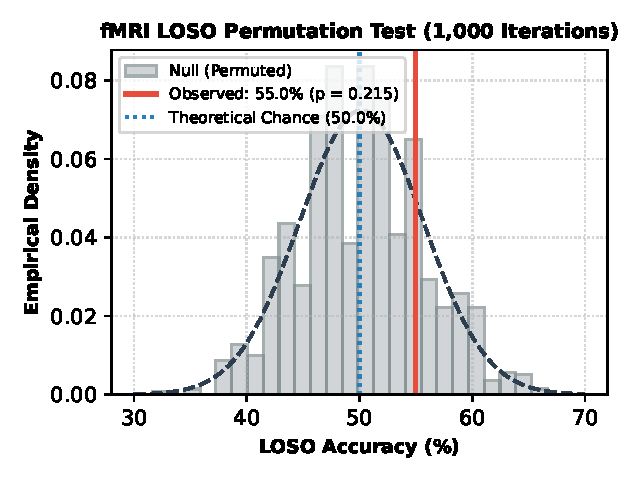
\includegraphics[width=0.80\linewidth]{figures/fig_loso_permutation.pdf}%
}{%
  \IfFileExists{figures/fig_loso_permutation.png}{%
    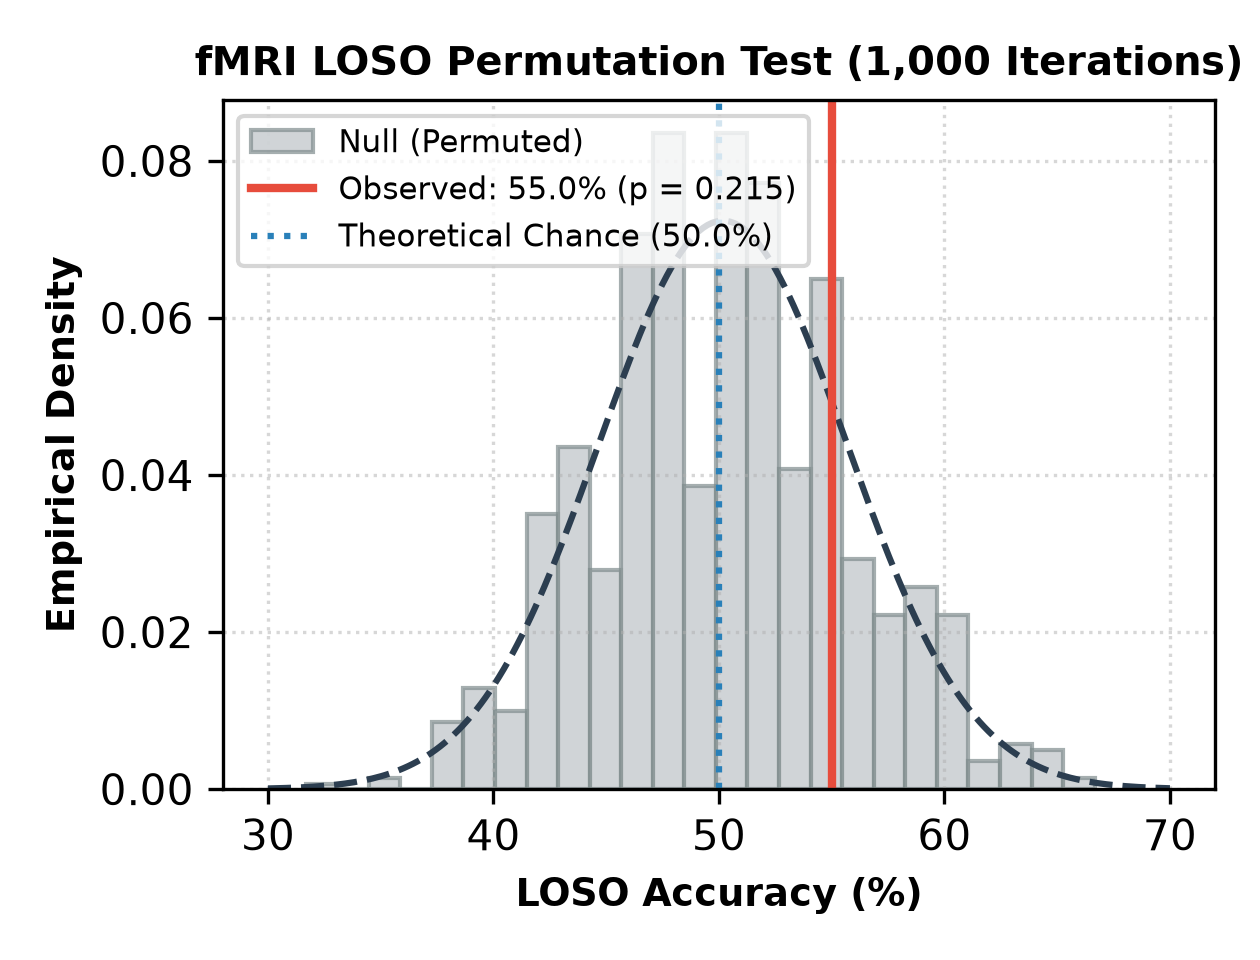
\includegraphics[width=0.80\linewidth]{figures/fig_loso_permutation.png}%
  }{%
    \fbox{\parbox[c][3.2cm][c]{0.80\linewidth}{\centering \footnotesize \textbf{Figure 1: Empirical Permutation Null Distribution}\\($B = 1{,}000$ permutations, mean 50.18\% $\pm$ 5.51\%, observed 55.00\%, $p = 0.215$)}}%
  }%
}
\caption{fMRI Leave-One-Site-Out (LOSO) empirical permutation null distribution across $B = 1{,}000$ within-site label permutations (mean \LosoWithinPermMean\,\% $\pm$ \LosoWithinPermSD\,\%), compared against observed primary pipeline accuracy (\LosoHeadlineAcc\,\%, one-sided $p = \LosoWithinPermP$) and theoretical chance ($50.0\,\%$).}
\label{fig:permutation}
\end{figure}

Fig.~\ref{fig:permutation} displays the empirical null distribution across $B = 1{,}000$ label permutations. In Protocol A (within-site label permutations preserving site marginals), the empirical null distribution had mean \LosoWithinPermMean\,\% $\pm$ \LosoWithinPermSD\,\%, yielding an empirical one-sided permutation $p$-value of $p = \LosoWithinPermP$. In Protocol B (global label permutations), the null distribution had mean \LosoGlobalPermMean\,\% $\pm$ \LosoGlobalPermSD\,\%, yielding an empirical one-sided permutation $p$-value of $p = \LosoGlobalPermP$.

To evaluate the influence of exploratory multiplicity, we catalogued all \NumFmriVariants\ evaluated fMRI model variants: (1) Primary LR Pipeline (`unseen\_rescaling'): \LosoHeadlineCorrect/\AbideTotalSubjects\ (\LosoHeadlineAcc\,\%, two-sided $p = \LosoBinomialPTwo$); (2) Unharmonized LR (`none'): \UnharmonizedCorrect/\AbideTotalSubjects\ (\UnharmonizedAcc\,\%, two-sided $p = 0.1203$); (3) Transductive Unlabeled Standardization: \TransductiveCorrect/\AbideTotalSubjects\ (\TransductiveAcc\,\%, two-sided $p = 0.1706$); (4) Covariate-Aware ComBat: \CovariateCombatCorrect/\AbideTotalSubjects\ (\CovariateCombatAcc\,\%, two-sided $p = 0.2352$); (5) Covariate-Regressed Connectome Model: \CovariateRegressedCorrect/\AbideTotalSubjects\ (\CovariateRegressedAcc\,\%, two-sided $p = 0.0824$); (6) Distilled Linear Student (\StudentEdges\ edges): \StudentCorrect/\AbideTotalSubjects\ (\StudentAcc\,\%, two-sided $p = 0.0548$); (7) Small Transformer Encoder Baseline (our implementation): \TransformerTestCorrect/\AbideTotalSubjects\ (\TransformerTestAcc\,\%, two-sided $p = \TransformerTestP$); (8) Random 10-Fold CV (non-site-held-out): \RandomTenFoldCorrect/\AbideTotalSubjects\ (\RandomTenFoldAcc\,\%, two-sided $p = 0.9273$); and (9) Site-Only Baseline: \SiteOnlyCorrect/\AbideTotalSubjects\ (\SiteOnlyAcc\,\%, two-sided $p = 0.6483$).
Across these \NumFmriVariants\ model variants, a Bonferroni-corrected significance threshold is $\alpha_{\text{Bonf}} = 0.05 / 9 = \BonferroniAlpha$. No variant meets family-wise significance. Observing an exploratory variant reaching \StudentAcc\,\% (\StudentCorrect/\AbideTotalSubjects) is fully consistent with expected sampling variability under multiple looks from the null. 

Furthermore, McNemar paired comparisons between the unharmonized baseline (`none`, \UnharmonizedAcc\,\%) and the alternative pipelines showed no detectable benefit from harmonization (differences of only 1--3 correctly classified subjects out of \AbideTotalSubjects): vs. `unseen\_rescaling` ($b=4, c=1$, exact $p = 0.3750$), vs. transductive ($b=7, c=6$, exact $p = 1.0000$), and vs. covariate-aware ($b=4, c=2$, exact $p = 0.6875$). Comparing the distilled student model (\StudentAcc\,\%) to the teacher model (\TeacherAcc\,\%) yielded a paired contingency table of 61 both correct, 5 teacher-only ($b$), 10 student-only ($c$), and 44 both incorrect (McNemar statistic \StudentTeacherMcnemarStat, exact two-sided $p = \StudentTeacherMcnemarP$).

A confound audit against phenotypic variables revealed no statistically significant correlation with model predicted likelihoods after Holm-Bonferroni adjustment across $N = \AbideTotalSubjects$: Age correlation was $r = \AgeCorrR$ (raw $p = \AgeCorrPRaw$, Holm $p = \AgeCorrPHolm$); head motion (mean framewise displacement) was $r = \MotionCorrR$ (raw $p = \MotionCorrPRaw$, Holm $p = \MotionCorrPHolm$); and sex was $r = \SexCorrR$ (raw $p = \SexCorrPRaw$, Holm $p = \SexCorrPHolm$). Regressing these three confounds inside training folds yielded \CovariateRegressedAcc\,\% LOSO accuracy (\CovariateRegressedCorrect/\AbideTotalSubjects).

The small Transformer encoder baseline (our implementation: 2 layers, $d_{\text{model}} = 64$, 4 attention heads, $d_{\text{ff}} = 128$, dropout 0.1, AdamW with learning rate $10^{-3}$, 12 epochs) achieved a mean training accuracy of \TransformerTrainAcc\,\%, but a LOSO test accuracy of \TransformerTestAcc\,\% (\TransformerTestCorrect/\AbideTotalSubjects, two-sided $p = \TransformerTestP$). This test performance illustrates the challenge of training multi-head attention architectures from scratch on small cohorts ($\sim 90$ training subjects per fold), where parameter count exceeds sample size.

Finally, an audit of scanner predictability confirmed that acquisition site is decodable from raw connectome edges under 5-fold cross-validation: pre-harmonization site classification achieved \PreCombatSiteAcc\,\% $\pm$ \PreCombatSiteSD\,\% accuracy (balanced accuracy \PreCombatSiteBAcc\,\%) against a majority-class baseline of \MajoritySiteBaseline\,\% (PITT) and balanced chance of \BalancedSiteChance\,\%.

% -----------------------------------------------------------------------
% Section V: Modular Client-Side Decision Support Prototypes
% -----------------------------------------------------------------------
\section{Modular Client-Side Decision Support Prototypes}

To evaluate engineering feasibility for privacy-preserving deployment, we investigated modular prototype components:

\subsection{Client-Side Conformal Triage for Questionnaires}
We formulated the split conformal prediction algorithm as a client-side triage design for the AQ-10. Because inference executes locally inside the user's web browser, responses can be scored on-device without transmitting data to remote servers. When an input item sum falls on the boundary ($\sum A_i \in \{6, 7\}$), the conformal layer outputs an empty set ($C = \emptyset$), displaying a calibrated alert: \textit{``Uncertain Presentation: Borderline screening score adjacent to referral threshold; specialist consultation recommended.''}

\subsection{Edge Deployment Exploration}
Edge deployment is left as future work. The conformal webapp is an engineering prototype designed for client-side triage.

% -----------------------------------------------------------------------
% Section VI: Discussion
% -----------------------------------------------------------------------
\section{Discussion}

Our findings demonstrate that high reported accuracies in public autism screening literature frequently reflect methodological vulnerabilities rather than genuine clinical breakthroughs.

\textbf{Behavioral Questionnaires:} Tabular screening benchmarks on public UCI and Kaggle repositories fit a deterministic step function. Machine learning models achieve 85.7\,\% to 100.0\,\% accuracy solely because the ground truth labels in these repositories were generated by thresholding the sum of the screening items ($\sum A_i \ge \tau$). Clinically, calculating $\sum A_i \ge \tau$ by hand is instant, deterministic, and 100.0\,\% concordant with repository labels, rendering complex supervised classifiers redundant. However, because this audit evaluated public repositories where ground truth was circular, it does not preclude machine learning from identifying non-linear phenotypic subtypes on prospective cohorts where independent gold-standard evaluations (e.g., ADOS-2, ADI-R) exist uncoupled from screening items.

\textbf{Multi-Site fMRI Connectomics:} On ABIDE-I, cross-site generalizability under Leave-One-Site-Out validation remains close to chance (\LosoHeadlineAcc\,\%). Our sample ($N = \AbideTotalSubjects$) has a lower point estimate (\LosoHeadlineAcc\,\%) and the study is underpowered below \LosoPowerMDE\,\% accuracy. Harmonization yields no detectable benefit; differences of only 1--3 subjects out of 120. Future consortium studies should scale Leave-Center-Out validation to the full consortium cohort across all 17 imaging sites.

% -----------------------------------------------------------------------
% Section VII: Conclusion
% -----------------------------------------------------------------------
\section{Conclusion}

This paper presented an empirical audit of machine learning for autism screening across behavioral questionnaires and multi-site resting-state fMRI. We established that near-perfect questionnaire classification in public benchmarks reflects circular label construction ($\sum A_i \ge \tau$, \ConcordancePct\,\% concordance across $N = \RetainedTotalCount$ records). In resting-state fMRI connectomics, strict Leave-One-Site-Out cross-validation yields \LosoHeadlineAcc\,\% accuracy (95\,\% CI: [\LosoWilsonLow\,\%, \LosoWilsonHigh\,\%]), which is statistically indistinguishable from chance under our sample size constraints. We developed modular prototypes for client-side decision support: split conformal prediction over 100 random splits achieves \ConformalMarginalCovMean\,\% $\pm$ \ConformalMarginalCovSD\,\% marginal coverage (\ConformalCZeroCovMean\,\% controls vs. \ConformalCOneCovMean\,\% ASD) while flagging borderline presentations, while edge deployment is left as future work. All evaluation scripts and preprocessing pipelines are available at \url{https://github.com/Mohit-ccreate/autism}.

% -----------------------------------------------------------------------
% References
% -----------------------------------------------------------------------
\bibliographystyle{IEEEtran}
\bibliography{references}

\end{document}
